\chapter{Практический раздел}

\section{Листинг алгоритма MD5}

\begin{lstlisting}[language=C, label=lst:md5, caption={Реализация алгоритма LZW на сжатие}]
void encode_lzw_data(FILE *f_in, FILE *f_out, dict_t *d) {
    uint8_t C = '\0';
    bytes_t P = {0};

    // Read data from file and create table dynamically.
    if (fread(&C, 1, 1, f_in)) {
        append_byte(&P, C);
        while (!feof(f_in)) {
            if (fread(&C, 1, 1, f_in)) {
                bytes_t temp = {0};
                append_bytes(&temp, P);
                append_byte(&temp, C);
                if (is_in_dict(d, temp)) {
                    copy_bytes(&P, temp);
                } else {
                    // Output the data for P.
                    short code = get_index(d, P);
                    write_byte_data(f_out, code, 0);
                    add_to_dict(d, temp);
                    copy_data(&P, C);
                }

                free_bytes(&temp);
            }
        }
        int code = get_index(d, P);
        write_byte_data(f_out, code, 0);
        // Write remaining data if any.
        write_byte_data(f_out, 0, 1);
    }
    free_bytes(&P);
}
\end{lstlisting}

\newpage

\begin{lstlisting}[language=C, label=lst:rsa, caption={Реализация алгоритма LZW на распаковку}]
void decode_lzw_data(FILE *f_in, FILE *f_out, dict_t *d) {
    short new;

    short old = get_lzw_code(f_in);
    bytes_t tmp = get_from_dict(d, old);
    bytes_t C = {0};
    bytes_t S = {0};

    fwrite(tmp.data, 1, tmp.len, f_out);
    copy_data(&C, tmp.data[0]);

    while ((new = get_lzw_code(f_in)) != -1) {
        if (d->data[new].len == 0) {
            S = get_from_dict(d, old);
            append_bytes(&S, C);
        } else {
            S = get_from_dict(d, new);
        }

        fwrite(S.data, 1, S.len, f_out);
        copy_data(&C, S.data[0]);
        tmp = get_from_dict(d, old);
        append_bytes(&tmp, C);
        add_to_dict(d, tmp);
        old = new;
    }
}
\end{lstlisting}

\section{Тестирование}

Корректность алгоритма проверялось путем применения дешифрации на шифрованное сообщение.

Тестирование было проведено на файлах с типами: текстовый (txt), графический (jpeg, png), архив (zip), несуществующий (ubc). Также, был проведен тест с повреждением зашифрованного файла.

В таблице \ref{tbl:test} представлены тестовые данные.

\begin{table}[H]
	\begin{center}
		\centering
		\caption{Тестовые данные}
		\label{tbl:test}
		\begin{tabular}{|c|c|c|} 
			
			\hline
			\multicolumn{1}{|c|}{Номер теста}
			&  \multicolumn{1}{c|}{Тип файла} &  \multicolumn{1}{c|}{Содержимое файла}\\
			\hline
			
			1& txt (1142.8572\%) &  {\specialcell{aaaa...}} \\ \hline
			
			2& ubc (0\%) &  $\varnothing$\\ \hline
			
			3& zip (68.7722\%) & Файлы с тестов 1, 2, 4 \\ \hline
			
			4& png (68.7669\%) & {\specialcell{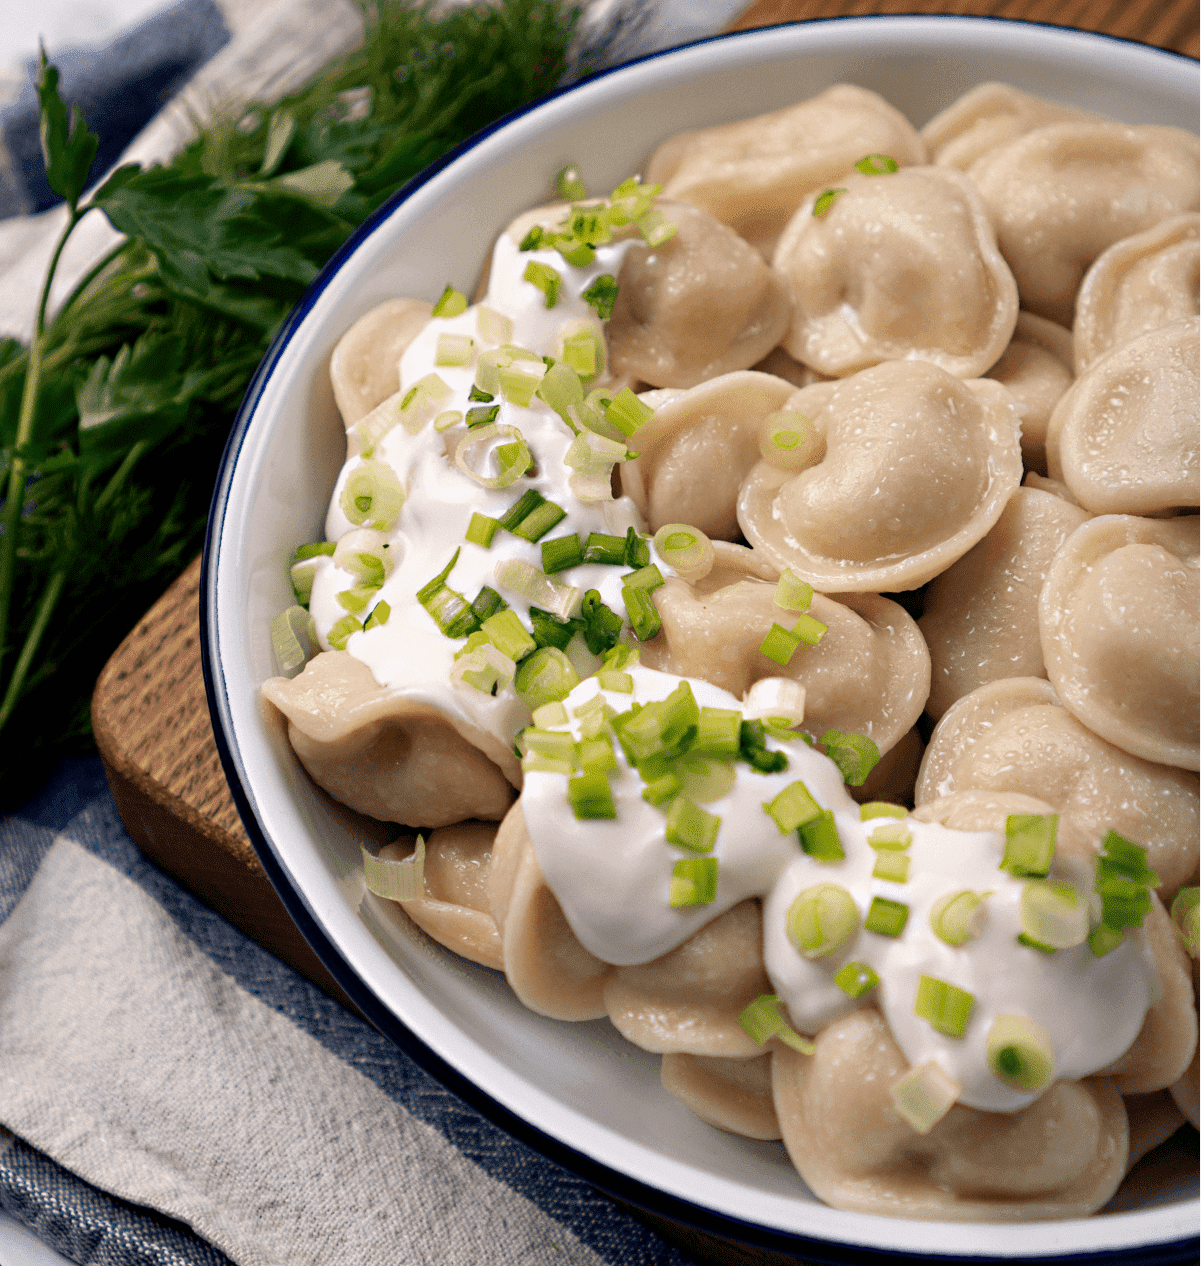
\includegraphics[width=1in]{assets/test4.png}}} \\ \hline
			
			5& bmp (5023.1802\%) & {\specialcell{
\includegraphics[width=1in]{assets/test10.pdf}}} \\ \hline
		
			
		\end{tabular}
	\end{center}
\end{table}

\newpage

\chapter*{ЗАКЛЮЧЕНИЕ}
\addcontentsline{toc}{chapter}{ЗАКЛЮЧЕНИЕ}

В результате выполнения данной лабораторной работы поставленная цель достигнута: реализована программа сжатия данных алгоритмом LZW.

В ходе выполнения лабораторной работы были выполнены все задачи.

\begin{enumerate}[label=\arabic*)]
	\item Изучен алгоритм LZW.
	\item Спроектирован алгоритм LZW.
	\item Реализован алгоритм LZW.
	\item Протестирована реализация алгоритма.
\end{enumerate}